\begin{frame}[plain]
  \begin{tikzpicture}[remember picture, overlay, shift={(current page.north west)}]

    \fill[argonneRed]
      (0.73mm, -0.77mm) rectangle ++(58.08mm, -5.81mm);
    \fill[argonneGreen]
      (2.18mm, -2.18mm) rectangle ++(72.59mm, -5.81mm);
    \fill[argonneBlue]
      (3.63mm, -3.63mm) rectangle ++(87.11mm, -5.81mm);
    \fill[white]
      (5.08mm, -5.08mm) rectangle ++(101.27mm, -7.30mm);

    \node[anchor=west,
          font=\fontsize{12}{14}\selectfont\bfseries,
          text width=96mm]
      at (7mm, -5.08mm - 7.30mm/2)
      {Timestep Trim Audit: 0.10 Threshold};

    \node[anchor=north west, inner sep=0pt]
      at (100mm, -3mm)
      {\includegraphics[width=25mm]{\argonneLogo}};

    \node[anchor=north west, inner sep=0pt]
      at (130mm, 1mm)
      {\includegraphics[width=25mm]{\atlasLogo}};

  \end{tikzpicture}

  \vspace{11mm}
  \centering
  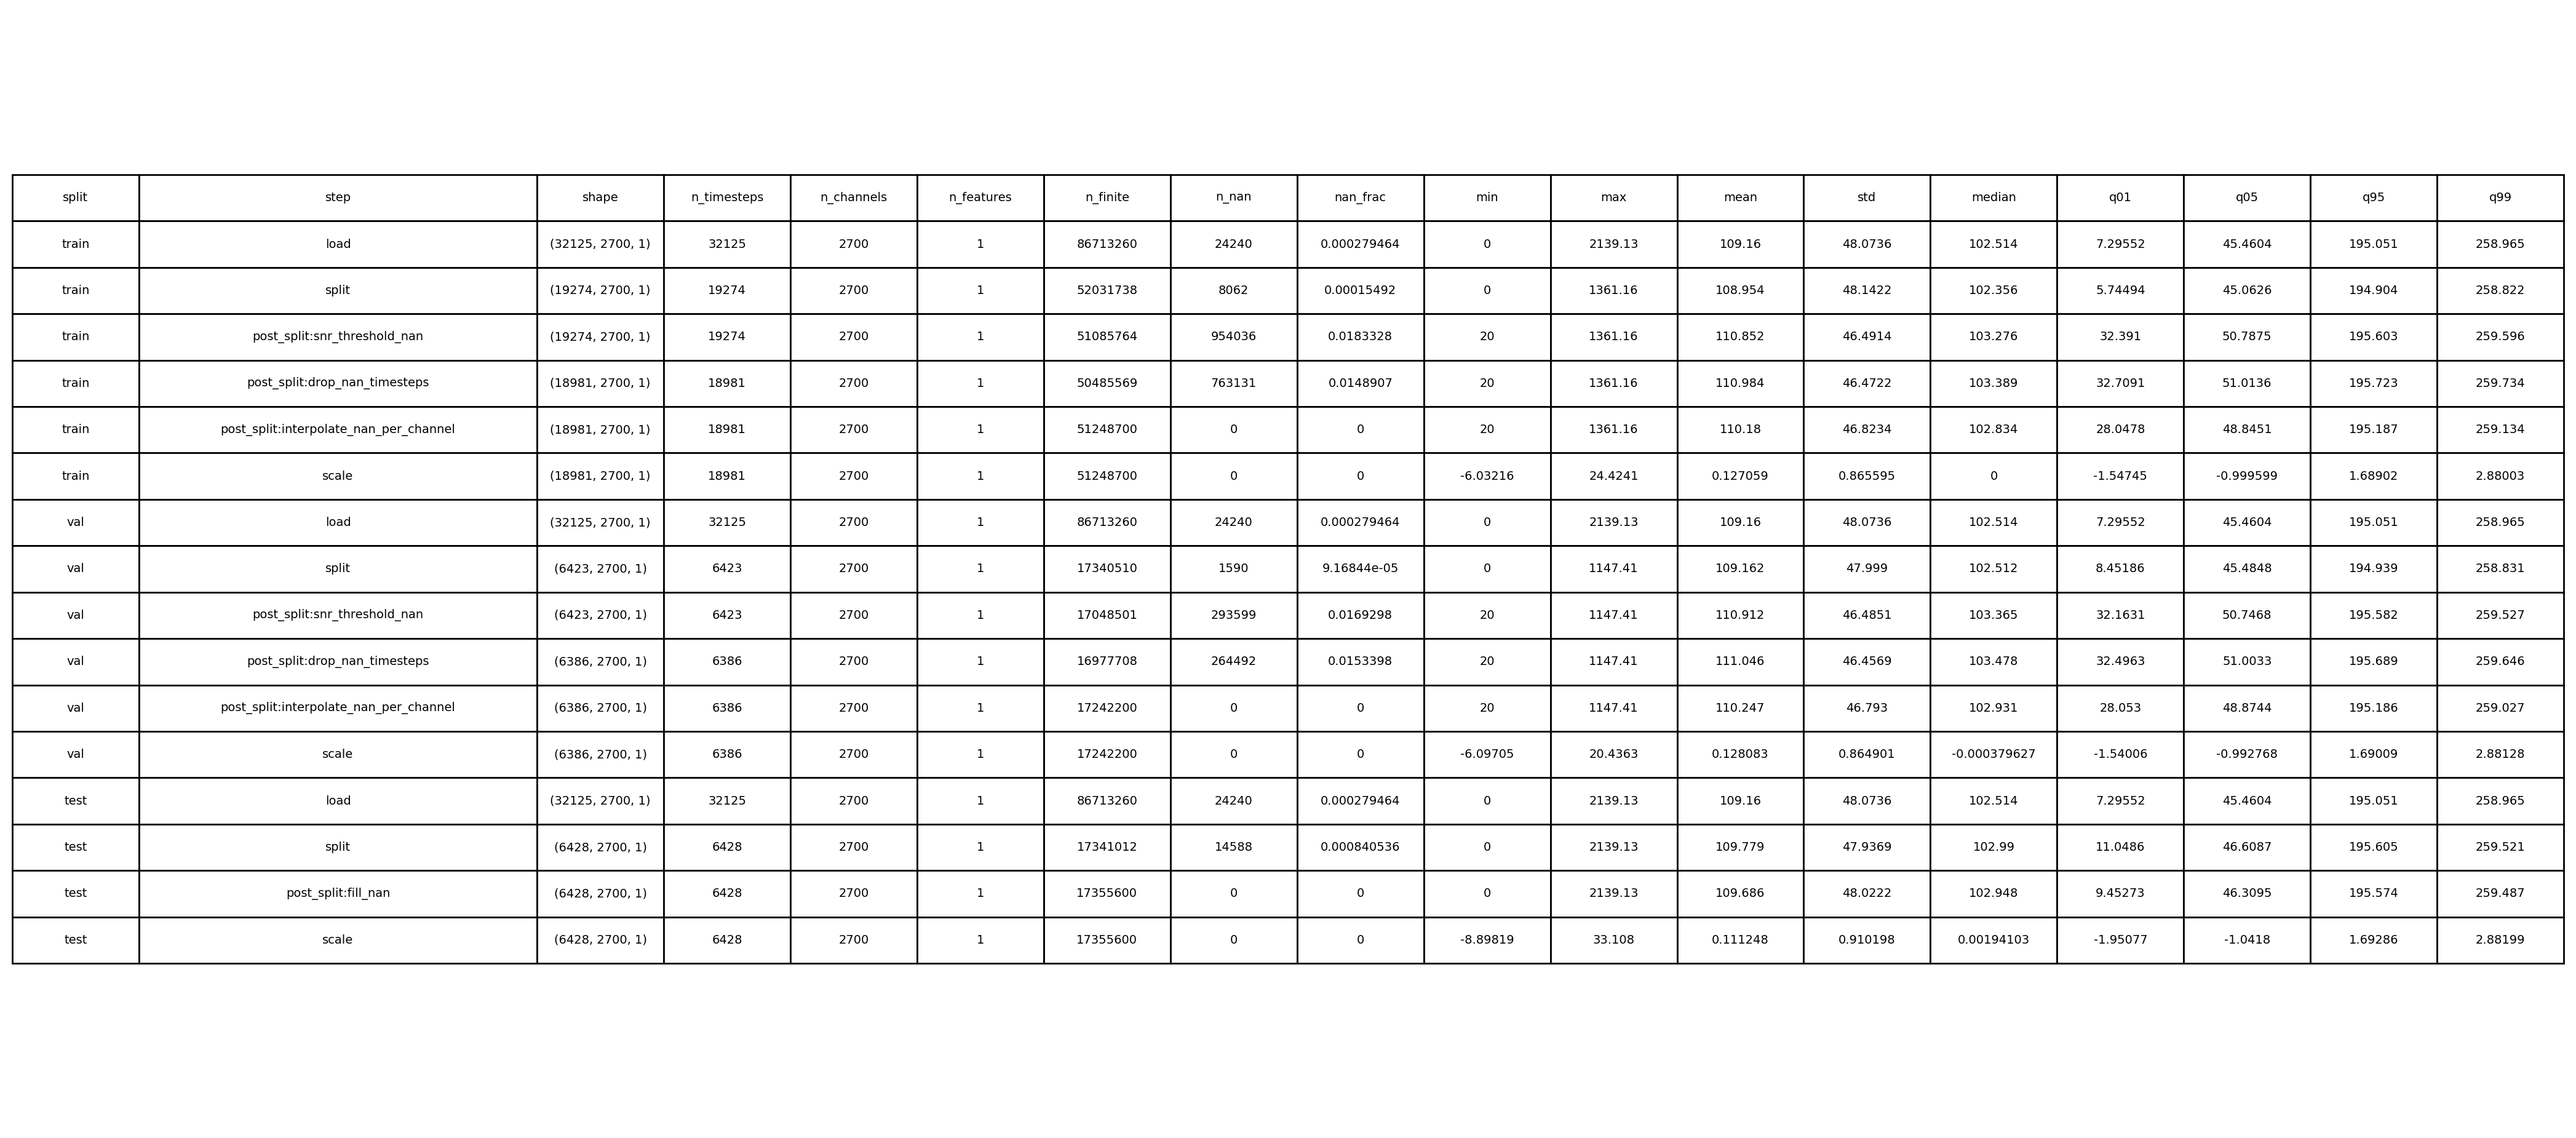
\includegraphics[width=0.95\textwidth,height=54mm,keepaspectratio]{figures/spt_timestep_trim_drop010_preprocessing_audit.png}

  \vspace{1.5mm}
  {\fontsize{8}{9.3}\selectfont
  \begin{center}
  \begin{minipage}{0.86\textwidth}
  {\setbeamertemplate{itemize item}{\color{black}-}
  \begin{itemize}
    \item Train/val kept: 18981 / 6386 (trimmed 1.5\% / 0.6\%).
    \item Very light trim: only about 1.5\% of train timesteps removed; distribution is nearly identical to the no-cut baseline.
  \end{itemize}}
  \end{minipage}
  \end{center}}

  \slideheaderfooter
\end{frame}
